% !TeX program = xelatex
% !TeX encoding = UTF-8
% !TeX TXS-program:compile = txs:///xelatex | txs:///xelatex
\documentclass[aspectratio=169, table, 12pt]{beamer}
% Preamble bersama seluruh slide mata kuliah ini.
% Dipanggil dari slides/sessionXX/sessionXX.tex tepat sesudah baris
% \documentclass[aspectratio=169, table, 12pt]{beamer}
% Paket tambahan yang hanya dibutuhkan satu sesi ditulis di berkas sesi itu.

\usepackage{colortbl}
\usepackage{xcolor}
\usepackage{listings}
\usepackage{tabularx}
\usepackage{booktabs}
\usepackage{tikz}
\usepackage{pgfplots}
\pgfplotsset{compat=1.18}
\usetikzlibrary{arrows.meta, positioning, calc, fit, shapes.geometric,
	shapes.multipart, backgrounds, matrix, chains, trees}

\makeatletter
\def\input@path{{../theme/}}
\makeatother
\graphicspath{{../theme/}{../../figures/}}
\usetheme{Pradita}

\definecolor{praditagreen}{RGB}{37, 113, 71}

% Tema membuat garis tabel berwarna putih. Dikembalikan agar tabel terbaca.
\arrayrulecolor{black}
\setlength{\arrayrulewidth}{0.5pt}

\lstdefinelanguage{yaml}{
	basicstyle=\ttfamily\scriptsize,
	keywordstyle=\color{blue}\bfseries,
	commentstyle=\color{gray}\itshape,
	stringstyle=\color{red},
	showstringspaces=false,
	breaklines=true,
	frame=lines,
	numbers=none,
	backgroundcolor=\color{lightgray!10},
	tabsize=2,
	morecomment=[l]{\#}
}

\lstdefinelanguage{json}{
	basicstyle=\ttfamily\scriptsize,
	stringstyle=\color{red},
	commentstyle=\color{gray},
	breaklines=true,
	showstringspaces=false,
	tabsize=2,
	numbers=none,
	frame=lines,
	backgroundcolor=\color{lightgray!10},
	string=[s]{"}{"}
}

\lstdefinelanguage{bash}{
	keywords={},
	basicstyle=\ttfamily\scriptsize,
	ndkeywords={docker, kubectl, helm, curl, git, terraform},
	ndkeywordstyle=\color{purple}\bfseries,
	sensitive=true,
	commentstyle=\color{gray},
	numbers=none,
	breaklines=true,
	frame=lines,
	backgroundcolor=\color{lightgray!10},
	tabsize=2,
	comment=[l]{\#},
	showstringspaces=false
}

\lstdefinelanguage{http}{
	keywords={GET, POST, PUT, PATCH, DELETE, HEAD, OPTIONS, HTTP},
	basicstyle=\ttfamily\scriptsize,
	keywordstyle=\color{blue}\bfseries,
	sensitive=true,
	numbers=none,
	breaklines=true,
	frame=lines,
	backgroundcolor=\color{lightgray!10},
	tabsize=2,
	showstringspaces=false
}

\subtitle{IT40613 · Digital Platform \& API Economy}
\author{\textbf{Alfa Yohannis}}


\title{\Huge Ekosistem dan\\ \vspace{10pt} Orkestrasi Mitra}
\date{Pertemuan 03}

\begin{document}
\frame{\titlepage}

\begin{frame}
  \frametitle{Isi Pertemuan}
  \vspace{14pt}
  \begin{columns}[t]
    \column{0.5\textwidth}
    {\small\tableofcontents[sections={1-3}]}

    \column{0.5\textwidth}
    {\small\tableofcontents[sections={4-7}]}
  \end{columns}
\end{frame}

\begin{frame}{\hfill}
  \centering
  \Huge{\textbf{Bila kontraknya sudah ada,\\mengapa pasien masih\\membawa hasil\\pemeriksaan sendiri?}}
\end{frame}

\section{Tujuan dan Konteks}

\begin{frame}{{\Large Tujuan Pembelajaran}}
  \vspace{10pt}
  \begin{itemize}
    \item Memetakan pelaku ekosistem, peran, dan aliran nilai di sekitar organisasi.
    \item Membandingkan opsi strategi platform, yaitu membangun, bergabung, atau bermitra, beserta
          \textit{tradeoff} masing-masing.
    \item Merumuskan aturan dasar keterbukaan platform bagi mitra.
  \end{itemize}
\end{frame}

\begin{frame}{{\Large Persoalan Medikara Health}}
  \vspace{10pt}
  \begin{itemize}
    \item Layanan ingin lintas fasilitas, tetapi hasil pemeriksaan masih dibawa pasien.
    \item Koneksi teknis tidak menjawab siapa melayani, siapa membayar, siapa menangani keluhan.
    \item Bab 2 memetakan sisi pasar. Bab ini memetakan seluruh pihak di sekitar platform.
    \item Angka berawalan ``Misalkan'' adalah asumsi latihan.
    \item Hasilnya menjadi bagian tonggak C1.
  \end{itemize}
\end{frame}

\begin{frame}{{\Large Diagram Konsep Bab 3}}
  \centering
  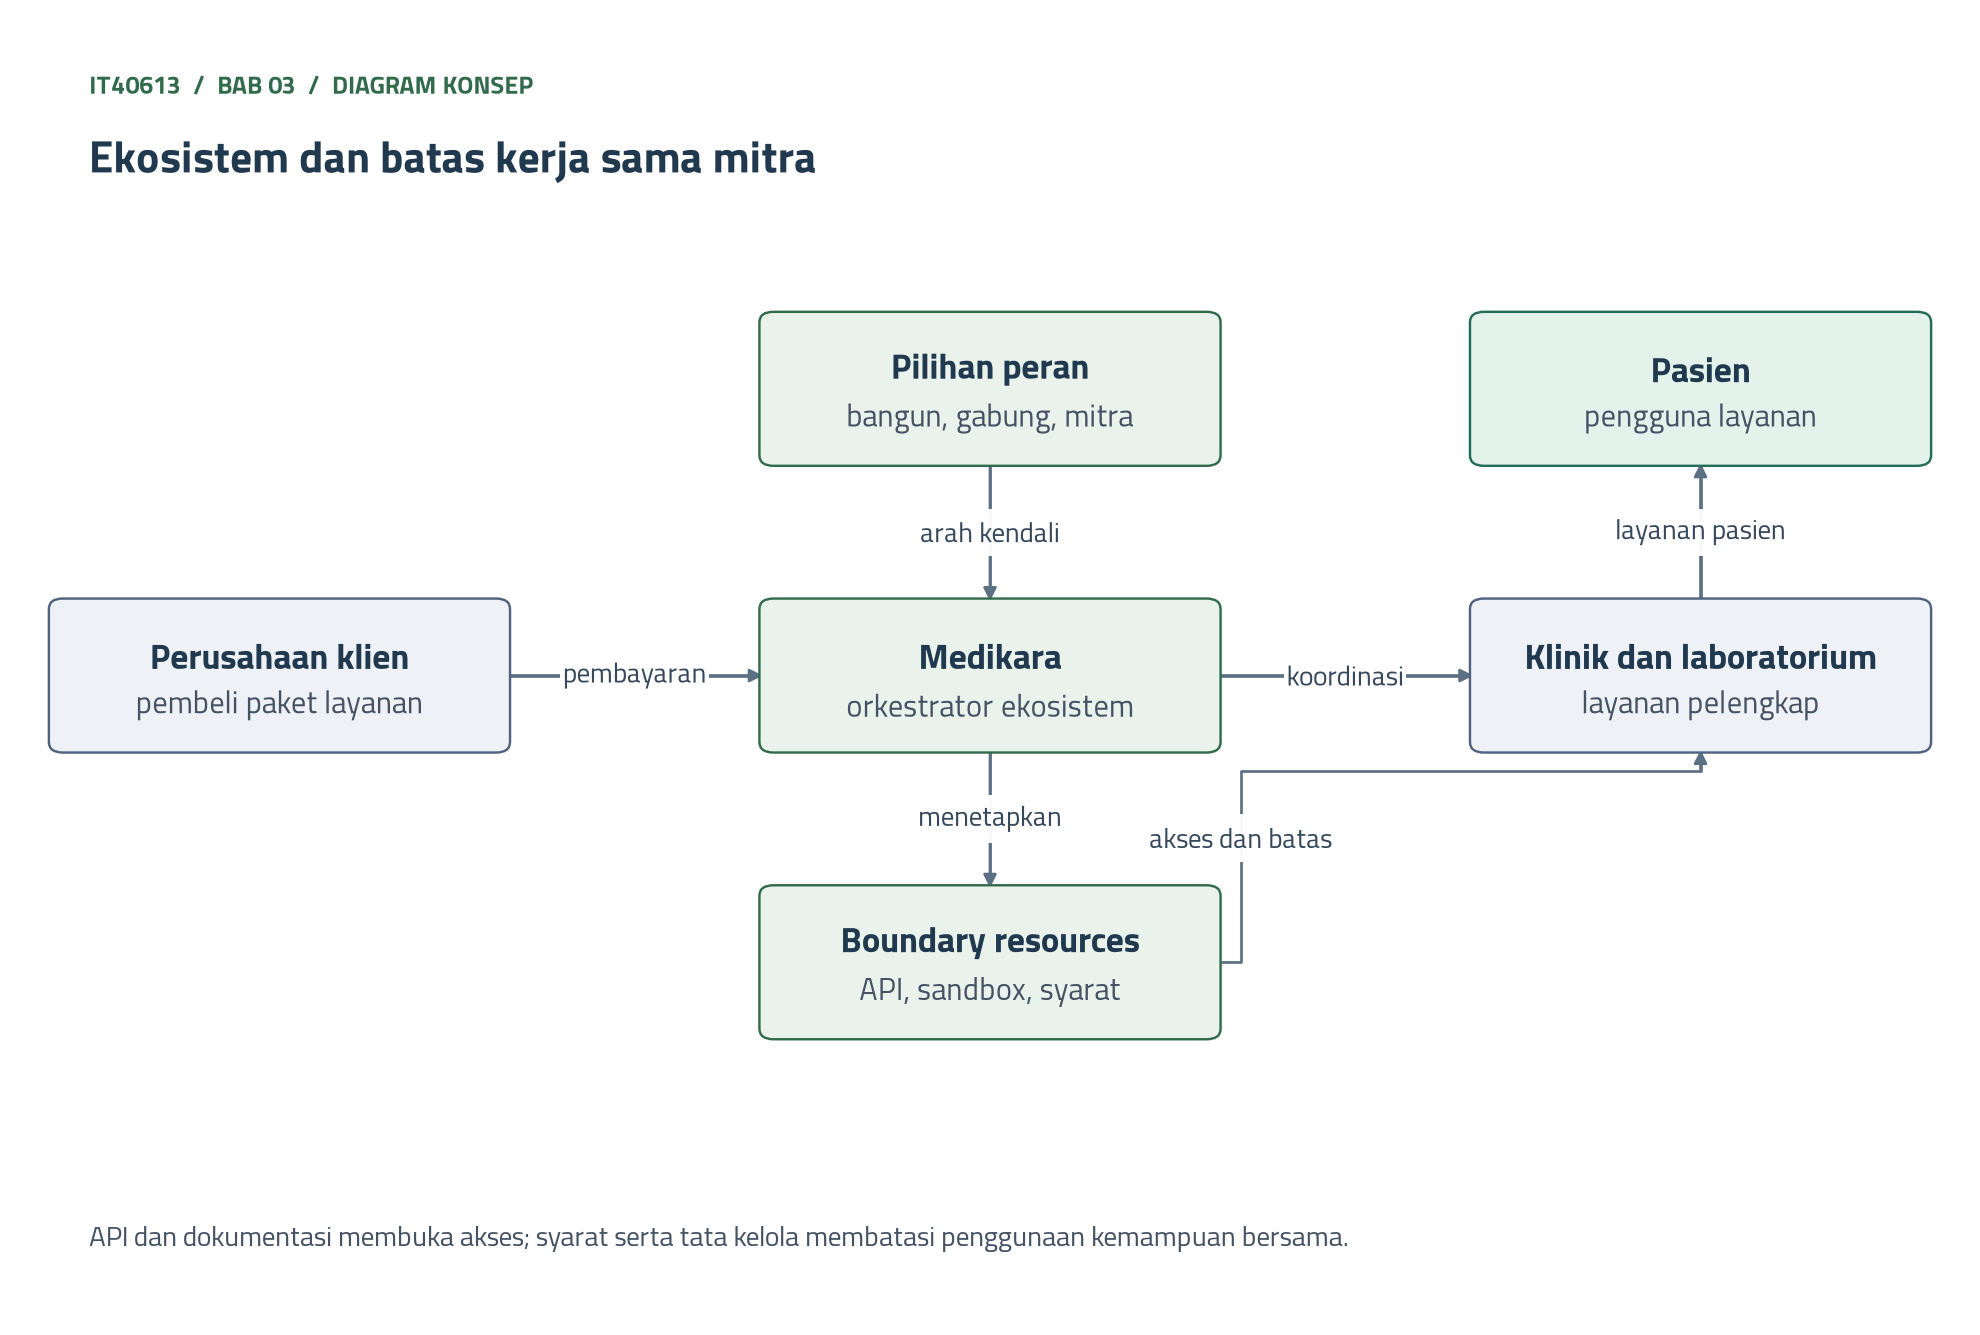
\includegraphics[width=0.96\textwidth,height=0.77\textheight,keepaspectratio]{../../figures/ch03-diagram-konsep.png}
\end{frame}

\section{Ekosistem}

\begin{frame}{\hfill}
  \centering
  \Huge{\textbf{Ekosistem sebagai\\Struktur Kerja Sama}}
\end{frame}

\begin{frame}{{\Large Apa Itu Ekosistem}}
  \vspace{10pt}
  \begin{itemize}
    \item Susunan pelaku yang saling melengkapi untuk satu tawaran nilai.
    \item Rantai pasok memakai kontrak khusus tiap pemasok; ekosistem memakai peran dengan aturan serupa.
    \item Jacobides dkk.: berinteraksi, dimungkinkan modularitas, tidak dikelola hierarkis.
    \item Adner: penyelarasan mitra agar satu tawaran nilai terwujud.
    \item Pemetaan dimulai dari tawaran nilai, bukan dari daftar mitra.
  \end{itemize}
  \vspace{6pt}
  {\small Analogi: paket perjalanan. Kamar bagus tidak menolong bila bus terlambat dua jam.}
\end{frame}

\begin{frame}{{\Large Tiga Unsur yang Diperiksa}}
  \footnotesize
  \begin{tabularx}{\textwidth}{>{\raggedright\arraybackslash}p{3.3cm}
      >{\raggedright\arraybackslash}X >{\raggedright\arraybackslash}X}
    \hline
    \textbf{Unsur} & \textbf{Contoh Medikara} & \textbf{Pertanyaan uji} \\ \hline
    Komplementaritas & Klinik dan laboratorium dalam satu perjalanan pasien & Apakah nilai satu pihak turun bila pihak lain tidak ada? \\ \hline
    Modularitas & Kontrak hasil pemeriksaan bersama & Dapatkah satu pihak berubah tanpa memaksa pihak lain berubah? \\ \hline
    Batas ekosistem & Mitra layanan aktif, bukan semua pemasok & Apakah hubungan ini punya tujuan bersama yang dapat diukur? \\ \hline
  \end{tabularx}

  \vspace{8pt}
  \small Unik: A tidak bekerja baik tanpa B. \textit{Supermodular}: makin banyak A, makin bernilai B.
\end{frame}

\begin{frame}{{\Large Dua Contoh Berangka}}
  \vspace{10pt}
  \begin{itemize}
    \item Misalkan 12 persen dari 1.100 pemeriksaan per bulan terlambat: 132 pasien menunggu.
    \item 7.800 klaim per bulan, 9 format, 6 persen ditolak: 468 klaim per bulan.
    \item Misalkan 40 klinik terhubung langsung ke 3 laboratorium: 120 sambungan.
    \item Satu kontrak bersama lewat Medikara+: 43 sambungan.
    \item Misalkan Rp4 juta per sambungan: Rp480 juta turun menjadi Rp172 juta per tahun.
  \end{itemize}
\end{frame}

\begin{frame}{{\Large Kasus Medikara: Sudah Punya Ekosistem?}}
  \vspace{10pt}
  \begin{itemize}
    \item 3 laboratorium, 9 asuransi, 36 perusahaan: 48 hubungan dengan cara sendiri.
    \item Kesimpulan: kumpulan hubungan dua pihak, belum ekosistem.
    \item Disusun ulang menjadi tiga peran: laboratorium mitra, penjamin, perusahaan klien.
    \item Konsekuensi pertama: merawat tiga set aturan, bukan 48 kebiasaan.
    \item Konsekuensi kedua: mitra kehilangan kelonggaran, perlu masa transisi.
  \end{itemize}
\end{frame}

\section{Peran dan Aliran Nilai}

\begin{frame}{\hfill}
  \centering
  \Huge{\textbf{Peran dan\\Aliran Nilai}}
\end{frame}

\begin{frame}{{\Large Orkestrator, Pelengkap, dan Pengguna}}
  \vspace{10pt}
  \begin{itemize}
    \item Orkestrator menetapkan aturan interaksi dan menjaga kesehatan ekosistem.
    \item Pelengkap (\textit{complementor}) menyediakan bagian layanan yang memperbesar nilai.
    \item Pengguna menerima atau memilih nilai tersebut.
    \item Misalkan paket 200 karyawan, Rp500.000 per karyawan: yang membayar bukan yang memakai.
    \item Asuransi: membayar Rp960 juta untuk verifikasi, sekaligus menyediakan penjaminan.
  \end{itemize}
  \vspace{6pt}
  {\small Analogi: pengelola pasar yang mulai membuka lapak sendiri.}
\end{frame}

\begin{frame}{{\Large Mitra dan Pelanggan Sering Tertukar}}
  \footnotesize
  \begin{tabularx}{\textwidth}{>{\raggedright\arraybackslash}p{3.3cm}
      >{\raggedright\arraybackslash}X >{\raggedright\arraybackslash}X}
    \hline
    \textbf{Aspek} & \textbf{Mitra} & \textbf{Pelanggan} \\ \hline
    Peran dalam nilai & Ikut menciptakan atau menyalurkan & Menerima dan memakai \\ \hline
    Arah uang & Dapat menerima atau membayar & Umumnya membayar \\ \hline
    Tanggung jawab mutu & Ikut menanggung, tertulis di perjanjian & Tidak menanggung \\ \hline
    Hak utama & Akses teknis, data sesuai tujuan, kepastian aturan & Layanan sesuai janji, jalur keluhan \\ \hline
    Contoh Medikara & Klinik mitra yang melayani paket karyawan & Perusahaan yang membeli paket untuk 200 karyawan \\ \hline
  \end{tabularx}

  \vspace{8pt}
  \small Klinik mitra membayar Rp3 juta per bulan, tetapi tetap mitra karena ikut menciptakan layanan.
\end{frame}

\begin{frame}{{\Large Peta Ekosistem Medikara+}}
  \centering
  \eadiagram{../../figures/ch03-peta-ekosistem.tex}
\end{frame}

\begin{frame}{{\Large Empat Aliran Nilai}}
  \footnotesize
  \begin{tabularx}{\textwidth}{>{\raggedright\arraybackslash}p{1.7cm}
      >{\raggedright\arraybackslash}X >{\raggedright\arraybackslash}X
      >{\raggedright\arraybackslash}p{3.0cm}}
    \hline
    \textbf{Aliran} & \textbf{Pertanyaan} & \textbf{Contoh Medikara} & \textbf{Ukuran} \\ \hline
    Uang & Siapa membayar siapa, dan berapa? & Paket Rp100 juta, dibagi tiga pihak & Porsi tiap pihak \\ \hline
    Data & Data apa, untuk tujuan apa, dengan hak apa? & Hasil ke klinik, rekap agregat ke perusahaan & Akses sesuai tujuan \\ \hline
    Layanan & Siapa melayani, dan siapa menangani keluhan? & Pemeriksaan di klinik mitra & Waktu hasil, keluhan \\ \hline
    Reputasi & Nama siapa yang naik atau turun? & Ulasan pada Medikara+ & Nilai ulasan per klinik \\ \hline
  \end{tabularx}

  \vspace{8pt}
  \small Analogi: hajatan dengan katering. Tamu mengeluh kepada tuan rumah, walaupun katering yang memasak.
\end{frame}

\begin{frame}{{\Large Aliran pada Paket 200 Karyawan}}
  \centering
  \eadiagram{../../figures/ch03-aliran-nilai.tex}
\end{frame}

\begin{frame}{{\Large Membaca Aliran dengan Angka}}
  \vspace{10pt}
  \begin{itemize}
    \item Dari Rp100 juta: klinik Rp70 juta, laboratorium Rp20 juta, Medikara+ Rp10 juta.
    \item Medikara memegang 10 persen uang, tetapi namanya tercantum pada paket.
    \item Misalkan 3 klinik (7,5 persen) menyumbang 120 dari 300 keluhan (40 persen).
    \item Reputasi sistem adalah aset bersama yang mengundang penumpang gelap.
    \item Data kesehatan bersifat spesifik: perusahaan hanya menerima rekap agregat.
  \end{itemize}
\end{frame}

\begin{frame}{{\Large Kasus Medikara: Tiga Sambungan Terlemah}}
  \vspace{10pt}
  \begin{itemize}
    \item Hasil laboratorium: 1.100 per bulan, surel pindaian, diketik ulang ke SIMRS.
    \item Klaim asuransi: 7.800 per bulan, 9 format, 468 ditolak.
    \item Rekap perusahaan: 36 per bulan, empat hari kerja, data beredar di surel.
    \item Yang dirugikan berbeda: pasien, bagian keuangan, dan karyawan.
    \item Ketiganya calon pertama API mitra, diurutkan menurut akibatnya (Bab 4).
  \end{itemize}
\end{frame}

\section{Boundary Resources dan Keterbukaan}

\begin{frame}{\hfill}
  \centering
  \Huge{\textbf{Boundary Resources\\dan Keterbukaan}}
\end{frame}

\begin{frame}{{\Large Membuka Sekaligus Membatasi}}
  \vspace{10pt}
  \begin{itemize}
    \item Sarana yang membuka partisipasi sekaligus membatasi perilaku mitra.
    \item \textit{Resourcing}: memindahkan kemampuan merancang ke pihak luar.
    \item \textit{Securing}: menjaga kendali pemilik atas platform.
    \item Dibuat untuk pengembang pihak ketiga, bukan diturunkan dari arsitektur.
    \item Terus dibentuk ulang: studi iOS, 30 sarana lewat 4.664 artikel blog.
  \end{itemize}
  \vspace{6pt}
  {\small Analogi: pintu, kartu akses, dan papan penunjuk arah di gedung kantor.}
\end{frame}

\begin{frame}{{\Large Posisi di antara Mitra dan Platform}}
  \centering
  \eadiagram{../../figures/ch03-boundary-resources.tex}
\end{frame}

\begin{frame}{{\Large Dua Contoh dan Konsekuensinya}}
  \vspace{10pt}
  \begin{itemize}
    \item Misalkan 3 hari per klinik: 40 klinik butuh 120 hari kerja, atau Rp57,6 juta pada tarif Rp60.000 per jam.
    \item Dengan panduan, setengah hari per klinik: 20 hari kerja, atau Rp9,6 juta.
    \item \textit{Sandbox}: 20 pasien sintetis, 6 skenario gagal, tanpa rekam medis produksi.
    \item Misalkan biaya sarana Rp150 juta: baru kembali setelah 125 klinik.
    \item Alasan yang lebih kuat adalah keamanan, karena data produksi tidak dipakai uji.
  \end{itemize}
\end{frame}

\begin{frame}{{\Large Kasus Medikara: Yang Sudah Ada dan yang Belum}}
  \footnotesize
  \begin{tabularx}{\textwidth}{>{\raggedright\arraybackslash}p{4.0cm}
      >{\raggedright\arraybackslash}p{1.8cm} >{\raggedright\arraybackslash}X}
    \hline
    \textbf{Sarana} & \textbf{Status} & \textbf{Catatan} \\ \hline
    Kontrak kerja sama & Sebagian & Ada untuk laboratorium, belum untuk klinik mitra \\ \hline
    API jadwal dan pemesanan & Belum & Vendor masih membaca basis data SIMRS langsung \\ \hline
    \textit{Sandbox} & Belum & Pengujian selama ini memakai salinan data \\ \hline
    Panduan dan contoh & Belum & Pengetahuan tersimpan pada dua staf integrasi \\ \hline
    Syarat penggunaan & Belum & Perlu disusun bersama bagian hukum \\ \hline
  \end{tabularx}

  \vspace{8pt}
  \small Contoh publik: SATUSEHAT punya panduan registrasi, survei keamanan, dan kode akses \textit{sandbox}.
\end{frame}

\begin{frame}{{\Large Memberi Akses, Melepas Kendali}}
  \vspace{10pt}
  \begin{itemize}
    \item Tiga dimensi: siapa boleh bergabung, data apa tersedia, aksi apa diperbolehkan.
    \item Boudreau: 21 sistem komputasi genggam, 1990 sampai 2004.
    \item Memberi akses mempercepat perangkat baru sampai lima kali lipat.
    \item Melepas kendali tetap positif, tetapi efek tambahannya satu orde lebih kecil.
    \item Buktinya dari industri lain: arahnya berguna, angkanya tidak dapat dipindahkan.
  \end{itemize}
  \vspace{6pt}
  {\small Analogi: katalog perpustakaan terbuka, peminjaman butuh kartu, koleksi langka butuh izin.}
\end{frame}

\begin{frame}{{\Large Tangga Keterbukaan Medikara+}}
  \centering
  \eadiagram{../../figures/ch03-tangga-keterbukaan.tex}

  \vspace{6pt}
  {\footnotesize Kuota: 1.500 kunjungan per bulan, 60 per hari, 3 panggilan per pemesanan, 180 panggilan, cadangan menjadi 300.}
\end{frame}

\begin{frame}{{\Large Kasus Medikara: Lima Aturan Dasar}}
  \footnotesize
  \begin{tabularx}{\textwidth}{>{\raggedright\arraybackslash}X >{\raggedright\arraybackslash}X
      >{\raggedright\arraybackslash}p{2.9cm}}
    \hline
    \textbf{Aturan} & \textbf{Penerapan} & \textbf{Pemilik} \\ \hline
    Buka menurut tindakan, bukan menurut pihak & Membaca jadwal dan membaca hasil diatur berbeda & Pemilik produk \\ \hline
    Akses mengikuti tujuan layanan & Hasil hanya bagi fasilitas yang melayani pasien itu & Petugas pelindungan data \\ \hline
    Naik tingkat lewat bukti & Lulus 6 skenario gagal, kontrak ditandatangani & Pemilik kemitraan \\ \hline
    Batas dapat diukur & Kuota 100 dan 300 panggilan per hari, jejak akses & Tim platform \\ \hline
    Akses punya masa berlaku & Tingkat 3 ditinjau tiap 90 hari & Pemilik kemitraan \\ \hline
  \end{tabularx}

  \vspace{8pt}
  \small Misalkan vendor membaca 140 tabel, padahal butuh 2: 138 tabel adalah risiko tanpa manfaat.
\end{frame}

\section{Tata Kelola, Envelopment, dan Opsi Strategi}

\begin{frame}{\hfill}
  \centering
  \Huge{\textbf{Tata Kelola, Envelopment,\\dan Opsi Strategi}}
\end{frame}

\begin{frame}{{\Large Tata Kelola: Siapa Memutuskan Apa}}
  \footnotesize
  \begin{tabularx}{\textwidth}{>{\raggedright\arraybackslash}p{2.7cm}
      >{\raggedright\arraybackslash}X >{\raggedright\arraybackslash}p{3.3cm}}
    \hline
    \textbf{Tahap} & \textbf{Aturan pokok} & \textbf{Pemilik} \\ \hline
    Masuk & Verifikasi izin dan kemampuan & Pemilik kemitraan \\ \hline
    Berjalan & Pemantauan mutu dan kesepakatan layanan & Pemilik layanan \\ \hline
    Pembagian nilai & Harga, komisi, dan subsidi diumumkan & Keuangan \\ \hline
    Data & Peran pengendali dan prosesor data, tujuan akses & Petugas pelindungan data \\ \hline
    Sengketa & Jalur eskalasi dan batas waktu & Komite kemitraan \\ \hline
    Keluar & Penyelesaian kasus aktif dan pencabutan akses & Pemilik kemitraan \\ \hline
  \end{tabularx}

  \vspace{8pt}
  \small Tiwana: pembagian hak keputusan, pengendalian, dan penetapan harga. Analogi: koperasi.
\end{frame}

\begin{frame}{{\Large Contoh Berangka dan Wasit Merangkap Pemain}}
  \vspace{10pt}
  \begin{itemize}
    \item Misalkan laboratorium 88 persen, kesepakatan 95 persen: perbaikan 30 hari.
    \item Dicabut mendadak: dua laboratorium lain naik dari 700 menjadi 1.100, atau 57 persen.
    \item Misalkan klinik keluar dengan 35 rujukan aktif: 30 hari, lalu akses dicabut.
    \item Misalkan klinik sendiri 31 persen dari 58 klinik, tetapi menerima 70 persen pemesanan.
    \item Keputusan: kriteria filter diumumkan, data dipisahkan, sebaran ditinjau tiap triwulan.
  \end{itemize}
\end{frame}

\begin{frame}{{\Large Platform Envelopment}}
  \footnotesize
  Penyedia platform masuk ke pasar platform lain dengan membundel fungsi, memanfaatkan pengguna yang sama.

  \vspace{6pt}
  \begin{tabularx}{\textwidth}{>{\raggedright\arraybackslash}p{2.9cm}
      >{\raggedright\arraybackslash}p{4.3cm} >{\raggedright\arraybackslash}X}
    \hline
    \textbf{Hubungan} & \textbf{Contoh Eisenmann dkk.} & \textbf{Misalkan pada Medikara+} \\ \hline
    Saling melengkapi & Windows Media Player terhadap RealPlayer & Aplikasi asuransi menambah pemesanan janji temu \\ \hline
    Pengganti lemah & Blockbuster terhadap Netflix & Telekonsultasi nasional menambah pemesanan klinik \\ \hline
    Tidak berkaitan & iPhone terhadap Gameboy & Transportasi daring menambah layanan kesehatan \\ \hline
  \end{tabularx}

  \vspace{8pt}
  \small Misalkan 10 dari 40 klinik pindah: pendapatan turun Rp360 juta per tahun, 25 persen dari Rp1,44 miliar.
\end{frame}

\begin{frame}{{\Large Membangun, Bergabung, atau Bermitra}}
  \footnotesize
  \begin{tabularx}{\textwidth}{>{\raggedright\arraybackslash}p{2.6cm}
      >{\raggedright\arraybackslash}X >{\raggedright\arraybackslash}X >{\raggedright\arraybackslash}X}
    \hline
    \textbf{Aspek} & \textbf{Membangun} & \textbf{Bergabung} & \textbf{Bermitra} \\ \hline
    Biaya awal & Rp3,6 miliar & Rp400 juta, integrasi & Rp600 juta, uji lima klinik \\ \hline
    Biaya berjalan & Rp2,4 miliar per tahun & Komisi Rp60 juta per bulan & 60 persen dari Rp2,4 miliar selama 30 bulan \\ \hline
    Total tiga tahun & Rp10,8 miliar & Rp2,56 miliar & Rp4,2 miliar \\ \hline
    Kendali pasien & Penuh & Terbatas & Bersama \\ \hline
    Risiko utama & Mitra sepi, kemampuan tim kurang & Aturan berubah, \textit{envelopment} & Koordinasi lambat, sengketa \\ \hline
  \end{tabularx}

  \vspace{8pt}
  \small Analogi: toko sendiri, sewa tempat di pusat belanja, atau gerai bersama. Angka adalah asumsi latihan.
\end{frame}

\begin{frame}{{\Large Volume Bukan Keuntungan}}
  \vspace{10pt}
  \begin{itemize}
    \item Misalkan 2.000 calon pengguna per bulan, tarif Rp250.000, komisi 12 persen: Rp60 juta.
    \item Margin pasien baru 40 persen, atau Rp100.000 per konsultasi.
    \item Titik impas: 600 pasien baru per bulan, yaitu 30 persen dari 2.000.
    \item Bila hanya 25 persen yang baru: rugi Rp10 juta per bulan walaupun volume naik.
    \item Uji lima klinik enam bulan, Rp600 juta: seperenam dari investasi Rp3,6 miliar.
  \end{itemize}
\end{frame}

\begin{frame}{{\Large Pemenang Berganti Bila Bobot Berubah}}
  \footnotesize
  \begin{tabularx}{\textwidth}{>{\raggedright\arraybackslash}X >{\raggedright\arraybackslash}p{3.6cm}
      >{\raggedright\arraybackslash}p{2.0cm} >{\raggedright\arraybackslash}p{2.0cm}
      >{\raggedright\arraybackslash}p{1.8cm}}
    \hline
    \textbf{Pandangan} & \textbf{Bobot} & \textbf{Membangun} & \textbf{Bergabung} & \textbf{Bermitra} \\ \hline
    Dasar & 25, 25, 20, 15, 15 & 3,15 & 2,95 & \textbf{3,25} \\ \hline
    Pasar lebih dahulu & 15, 15, 40, 15, 15 & 2,35 & \textbf{3,65} & 3,15 \\ \hline
    Kendali lebih dahulu & 35, 35, 10, 10, 10 & \textbf{3,90} & 2,35 & 3,35 \\ \hline
  \end{tabularx}

  \vspace{8pt}
  \small Urutan bobot: kendali pasien, kendali data, kecepatan, biaya, kemampuan tim. Selisih 0,10 lebih kecil
  daripada keraguan saat memberi skor. Matriks memindahkan perdebatan ke kriteria.
\end{frame}

\begin{frame}{{\Large Peta Keputusan per Lapisan}}
  \centering
  \eadiagram{../../figures/ch03-peta-keputusan.tex}
\end{frame}

\begin{frame}{{\Large Kasus Medikara: Satu Keputusan per Lapisan}}
  \footnotesize
  \begin{tabularx}{\textwidth}{>{\raggedright\arraybackslash}p{4.0cm}
      >{\raggedright\arraybackslash}p{2.0cm} >{\raggedright\arraybackslash}X}
    \hline
    \textbf{Lapisan} & \textbf{Opsi} & \textbf{Pemicu tinjau} \\ \hline
    Identitas pasien, izin, API mitra & Membangun & Dua kali gagal audit akses \\ \hline
    Jaringan klinik dan laboratorium & Bermitra & Kurang dari 30 klinik aktif pada Gerbang 2 \\ \hline
    Kanal peserta asuransi & Bergabung & Pasien baru di bawah 30 persen selama tiga bulan \\ \hline
    Kesehatan karyawan & Bermitra & Rekap belum selesai dalam satu hari kerja \\ \hline
  \end{tabularx}

  \vspace{8pt}
  \small Syarat bergabung: tidak eksklusif, data layanan lanjutan sesuai izin pasien, hak keluar 90 hari.
\end{frame}

\section{Aktivitas}

\begin{frame}{{\Large Aktivitas: Peta Ekosistem dan Keputusan Strategi}}
  \vspace{6pt}
  \begin{itemize}
    \item Mulai dari kanvas Bab 2 dan daftar pertukaran data Bab 1: satu tawaran nilai.
    \item Gambar pelaku dan aliran; tandai tiga sambungan terlemah menurut akibatnya.
    \item Anggota teknis menandai \textit{boundary resources} yang ada dan yang belum.
    \item Sepakati bobot sebelum memberi skor, lalu uji paling sedikit dua set bobot lain.
    \item Tulis aturan keterbukaan dan catatan keputusan satu halaman.
  \end{itemize}
  \vspace{4pt}
  {\footnotesize Berkas: \berkas{sources/chapter03/README.md}. Data organisasi nyata wajib seizin dan dianonimkan.}
\end{frame}

\begin{frame}{{\Large Aktivitas: Peran, Luaran, dan Penilaian}}
  \vspace{6pt}
  \begin{itemize}
    \item Bisnis, manajemen, hukum, kesehatan: memimpin analisis peran dan kepentingan.
    \item Ilmu komputer, rekayasa perangkat lunak, TI: menelaah sarana.
    \item Akuntansi, keuangan: menyusun biaya dan uji bobot.
    \item Luaran C1: peta ekosistem, matriks opsi, aturan keterbukaan, catatan keputusan.
    \item Bobot: konsep 25, bukti 30, alasan dan pengorbanan 30, keterbacaan 15 persen.
  \end{itemize}
\end{frame}

\section{Ringkasan dan Latihan}

\begin{frame}{{\Large Ringkasan}}
  \vspace{10pt}
  \begin{itemize}
    \item Komplementaritas, modularitas, dan peran dengan aturan serupa membentuk ekosistem.
    \item Mitra dibedakan dari pelanggan oleh perannya menciptakan nilai, bukan arah uang.
    \item Keterbukaan adalah tangga: setiap kenaikan menuntut bukti baru.
    \item Tata kelola menetapkan siapa memutuskan apa, dari mitra masuk sampai keluar.
    \item Keputusan diambil per lapisan, beserta pengorbanan dan pemicu tinjau.
  \end{itemize}
\end{frame}

\begin{frame}{{\Large Latihan}}
  \vspace{10pt}
  \begin{enumerate}
    \item Jelaskan perbedaan mitra dan pelanggan dalam ekosistem layanan kesehatan, dengan satu contoh untuk
          masing-masing.
    \item Misalkan sebuah perusahaan asuransi mengajak Medikara bergabung ke platform milik asuransi tersebut.
          Analisis untung dan ruginya bagi Medikara dibandingkan membangun platform sendiri.
    \item Tentukan tiga \textit{boundary resources} yang perlu disediakan agar klinik mitra dapat terhubung tanpa
          pendampingan intensif.
  \end{enumerate}
\end{frame}

\end{document}
